\chapter{Izvođenje i rezultati}
\label{ch:rezultati}

\section{Primjer izvođenja programa}
\label{sec:izvodjenje}

Program se pokreće iz naredbenog retka naredbom \lstinline!./inverseMapping! kao u prikazu koda \ref{code:pokretanje}.
\begin{lstlisting}[label={code:pokretanje}, caption={Pokretanje programa}]
./inverseMapping originalna_slika.jpg transformirana_slika.jpg sirina_transfomirane_slike visina_transformirane_slike
\end{lstlisting}

Nakon toga se prikazuje prozor s originalnom slikom kao na slici \ref{fig:odabirTocaka1} na kojemu korisnik pokazivačem odabere četiri točke koje predstavljaju kutove dijela slike nad kojim je potrebno obaviti inverznu perspektivnu transformaciju, počevši od lijevog gornjeg u smjeru kazaljke na satu (slika \ref{fig:odabirTocaka2}).

\begin{figure}[ht]
\centering

\begin{subfigure}{0.45\textwidth}
\begin{minipage}{0.9\textwidth}
	\centering
	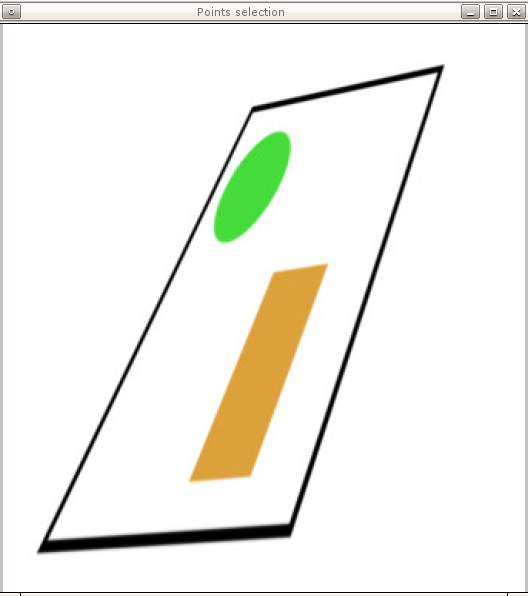
\includegraphics[width=\textwidth]{figures/points_selection.jpg}
	\caption[margin=1cm]{Originalna slika prije odabira točaka}
	\label{fig:odabirTocaka1}
\end{minipage}
\end{subfigure}%
\begin{subfigure}{0.45\textwidth}
\begin{minipage}{0.9\textwidth}
	\centering
	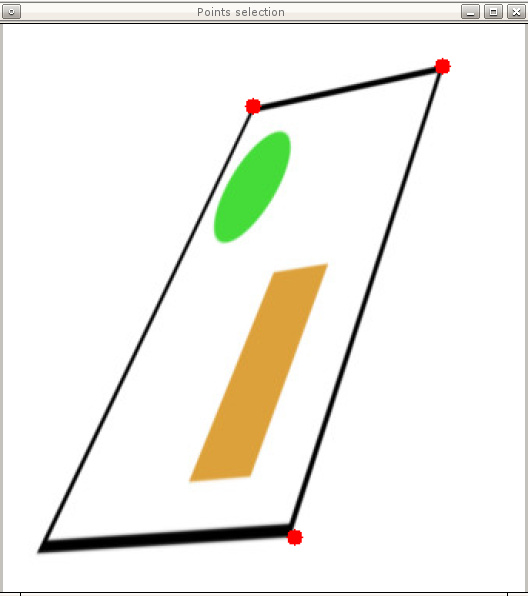
\includegraphics[width=\textwidth]{figures/points_selection_selected.jpg}
	\caption{Originalna slika za vrijeme odabira točaka}
	\label{fig:odabirTocaka2}
\end{minipage}
\end{subfigure}

\caption{Odabir točaka}
\label{fig:odabirTocaka}

\end{figure}

Nakon odabira točaka počinje izračunavanje transformacijske matrice, a nakon toga i sama transformacija slike čiji se napredak može pratiti u konzoli. Kada su svi slikovni elementi transformirani, transformirana se slika sprema u datoteku navedenu u naredbenom retku, a istovremeno se korisniku prikaže prozor s rezultatom, tj. istom tom transformiranom slikom (slika \ref{fig:transformiranaSlika}).

\begin{figure}[ht]
	\centering
	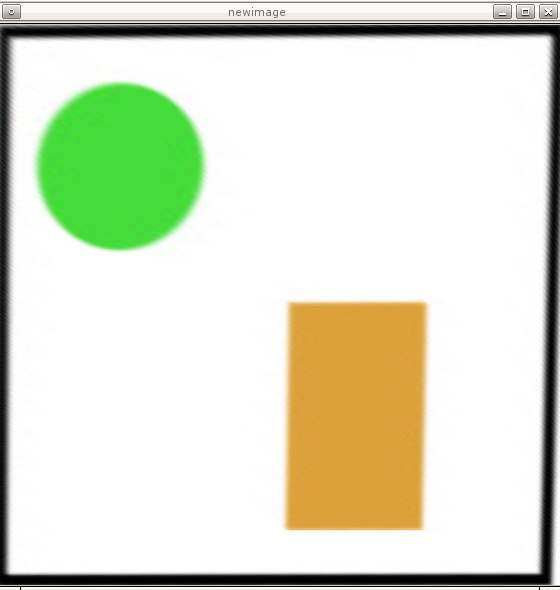
\includegraphics[width=0.7\textwidth]{figures/transformedImage.jpg}
	\caption{Rezultantna slika nakon transformacije}
	\label{fig:transformiranaSlika}
\end{figure}

Program završava pritiskom na tipku <ESC>

\section{Rezultati}
\label{sec:rezultati}

Kao što je već bio navedeno u potpoglavlju \ref{ch:implementacija} najprije je razvijen prototip u jeziku Python, a zatim, kako bi se dobile zadovoljavajuće performanse program je implementiran u C++-u. Usporedbe brzine izvođenja se mogu vidjeti u tablici \ref{table:brzine}.

%\begin{savenotes}
\begin{table}[ht]
\caption{Brzine izvođenja programa u Pythonu i u C++-u}
\label{table:brzine}
\centering
\begin{tabular}{ | c | c | c | c | }
\hline\hline
Jezik & Rezolucija & Interpolacija & Vrijeme transformacije (ms) \\
%
\hline
C++ & 100x100 & NE & 20 \\
C++ & 100x100 & DA & 31 \\
C++ & 1000x1000 & NE & 1948 \\
C++ & 1000x1000 & DA & 3095 \\
C++ & 3000x3000 & DA & 32541 \\
Python & 10x10 & NE & 43 \\
Python & 10x10 & DA & 45 \\
Python & 100x100 & NE & 3478 \\
Python & 100x100 & DA & 4315 \\
Python & 500x500 & NE & 228945 \\
\hline
\end{tabular}
\end{table}
%\end{savenotes}

Vrijeme izračuna same transformacijske matrice nije navedeno u tablici jer ne ovisi niti o rezoluciji slike niti o tome radi li se interpolacija ili ne te je ono približno jednako $780 \mu s$ za Python program, a oko $130\mu s$ za C++ program. Mjerenja su provedena sa svim dijagnostičkim ispisima isključenima te s \emph{niceness}\footnote{nice je *nix program koji služi za promjenu \emph{niceness} vrijednosti, a pomoću koje onda kernel određuje prioritet procesa. \emph{Niceness} može poprimiti vrijednosti od -20 do 19 ili 20, s time da veći broj označava manji prioritet. Procesi na Linuxu se uglavnom automatski pokreću s \emph{niceness} vrijednosti 0.} vrijednosti -20, kako bi se što preciznije moglo izmjeriti vrijeme potrebno za samu transformaciju.

Ovi bi se rezultati mogli dodatno poboljšati raznim optimizacijama algoritma za transformaciju točaka, odnosno množenje matrica.

U nastavku je prikazano nekoliko primjera izlaznih slika. Ulazna slika je slika iz primjera \ref{fig:odabirTocaka1}, originalnih dimenzija 339x369px (uključujući bjelinu). Na slici \ref{fig:primjer3_noint} se može vidjeti rezultat perspektivne transformacije na sliku dimenzija 200x200px bez interpolacije, a na slici \ref{fig:primjer3_int} s interpolacijom.

\begin{figure}[ht]
\centering

\begin{subfigure}{\textwidth}
	\centering
	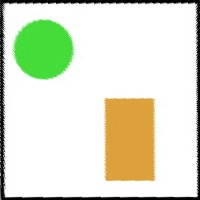
\includegraphics[scale=1]{figures/sample3_200_noint.jpg}
	\caption{Bez interpolacije}
	\label{fig:primjer3_noint}
\end{subfigure}
\begin{subfigure}{\textwidth}
	\centering
	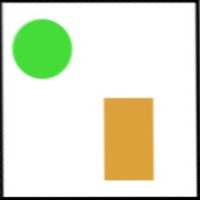
\includegraphics[scale=1]{figures/sample3_200_int.jpg}
	\caption{S interpolacijom}
	\label{fig:primjer3_int}
\end{subfigure}

\caption{Rezultat perspektivne transformacije}
\label{fig:primjer3}
\end{figure}

Nedostatak u pristupu ovog programa je način odabira točaka, budući da je potrebno pokazivačem točno pogoditi kut željenog dijela slike, što se često pokaže kao veoma težak zadatak. Kako bi se korisniku olakšalo rukovanje programom, moglo bi se drugim algoritmima (npr. \emph{Harrisov algoritam za detekciju kutova} odrediti sva potencijalna područja interesa, odnosno kutove, te bi korisnik trebao pokazivačem pogoditi samo relativnu blizinu kuta, ali ne i sam kut, nego bi taj dio posla program odradio za njega.

\clearpage
\section{Druge primjene}
\label{sec:drugePrimjene}

Budući da program radi perspektivnu transformaciju, a ne nužno ``ispravljanje" perspektive, moguće je ``dodati" perspektivu na postojeću sliku (slika \ref{fig:lipsum}).

\begin{figure}[ht]
\centering
\begin{subfigure}{0.45\textwidth}
\begin{minipage}{0.9\textwidth}
	\centering
	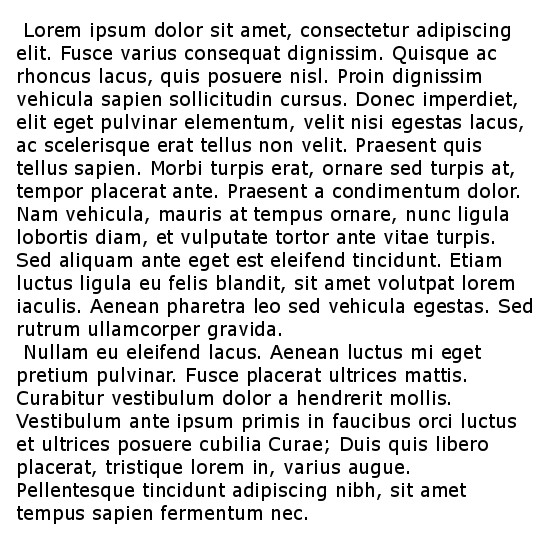
\includegraphics[width=\textwidth]{figures/lipsum.jpg}
	\caption{Originalna slika}
	\label{fig:lipsum_orig}
\end{minipage}
\end{subfigure}%
\begin{subfigure}{0.45\textwidth}
\begin{minipage}{0.9\textwidth}
	\centering
	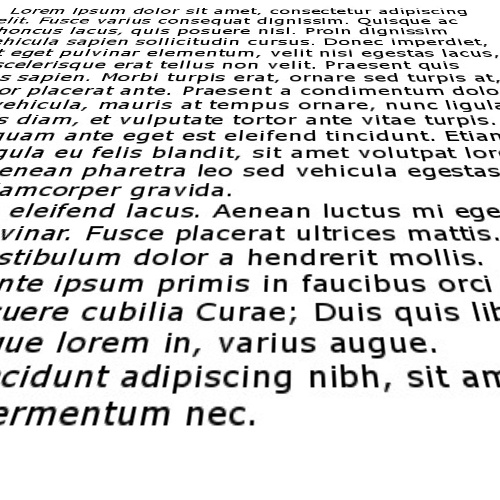
\includegraphics[width=\textwidth]{figures/lipsumPerspective.jpg}
	\caption{Transformirana slika na koju je "dodana" perspektiva}
	\label{fig:lipsumPerspective}
\end{minipage}
\end{subfigure}
\caption{"Dodavanje" perspektive na sliku}
\label{fig:lipsum}

\end{figure}
